\documentclass[12pt]{article}
\usepackage{amsmath} % flere matematikkommandoer
\usepackage[utf8]{inputenc} % æøå
\usepackage[T1]{fontenc} % mere æøå
\usepackage[danish]{babel} % orddeling
\usepackage{verbatim} % så man kan skrive ren tekst
\usepackage[all]{xy} % den sidste (avancerede) formel i dokumentet
\usepackage{graphicx}
\usepackage{listings}
\usepackage{url}
\title{ProjektKursus Systemudvikling 2014\\Delrapport 4}
\author{}

\begin{document}
\maketitle
\noindent{Gruppemedlemmer:}\\
Kenneth Christensen: 02 08 93\\Michael Jensen: 01 07 93\\Rune Pedersen: 01 11 82\\Rasmus Hansen: 03 12 92
\\\\
Instructor: Kasper Passov

\pagebreak
\section{Abstract}
We have choosen to work on a project for a local bike shop called "bmx-butikken". Bmxbutikken is specialised in the freestyle BMX community. They sell all you need as a BMX rider, which is everything from cloths and shoes to complete bikes and parts. They have a phsyical shop on Nørrebrogade, and a webshop at \url{www.bmxbutikken.dk}. The project regards a Spotguide app for all devices, programmed as a web application. This site is supposed to help local riders to find new places to ride, and foreigners to find any places to ride and hook up with the local crew. The app can also show you where bmx-butikken is located if you need a spare part. The application is designed for all bmx riders mainly in Copenhagen, but spots can be uploaded from anywhere.
\section{IT-projektets formål og rammer}
Følgende model er en FACTOR analyse af projektet og giver en kort og konkret beskrivelse af rammerne for projektet.\\

\begin{raggedleft}
  \begin{tabular}{| l | l |}
    \hline
    Funktionalitet & Give oplysninger om bmx spots\\ & Give oplysning om specialiserede bmx butikker\\ & Give rutevejledning\\ \hline
    Application Domain & BMX udøverer og bmxbutikkens kunder\\ \hline
    Conditions & Hjemmesiden skal kunne køres på smartphones\\ & Åben internet forbindelse \\ & Adgang til din lokation\\
    \hline
        Technology & HTML \\ & Javascript \\ & CSS\\ & mySQL\\ & PHP\\
    \hline
        Objects & Skate Spots\\ & Shops\\ & BMX Spots\\
    \hline
        Responsibilities & Give information om spots og rutevejleding \\ & Informerer om selve bmxbutikken\\
    \hline
  \end{tabular}
\end{raggedleft}


\pagebreak

\section{Kravspecifikation for IT-løsningen}
\subsection*{Funktionelle krav}
\textbf{Add spot} \\ Tilføjer et spot til Databasen hvor der måske kan være et billede med.\\
\textbf{Menu}\\ Indeholder 5 ting du kan trykke på der kan vejlede bruger: Spots, shops, settings, Add spot, Search\\
\textbf{Streetspots}\\ Viser brugeren en liste over de forskellige spots.\\
\textbf{Markers}\\ Viser på kortet 3 ting: Brugerens lokation, spots og bmxbutikkens lokation\\
\textbf{Rutevejledning}\\ Vejleder brugeren til det pågældende punkt på kortet ved hjælp af google maps.\\
\textbf{Bruger lokation}\\ Finder brugerens lokation.\\
\textbf{Shops}\\ Centrerer kortet på bmxbutikken.
\subsection*{Ikke funktionelle krav:}
\textbf{Sprog}\\ Siden skal være på engelsk, så den kan bruges af turister, men samtidig af de lokale da de fleste i miljøet snakker engelsk.\\
\textbf{Bruger venligt UI}\\ Nemt og intuitivt for brugeren at komme rundt.\\
\subsection*{Constraints}
Systemet skal være kompatibelt med både computere og telefoner.[Implementation requirement]\\
Kortet skal vise en marker ved bmxbutikken[User Interface Requirement]\\
Koden skal være skrevet i php/javascript/html/mysql.[Implementation requirement]\\
\pagebreak\\

\textit{(b) En use case model, der beskriver system-funktionaliteten. Der ønskes et højniveau-diagram,
som giver overblik over hvilke use cases de forskellige aktører har}\\
\begin{figure}[htb]
\begin{center}
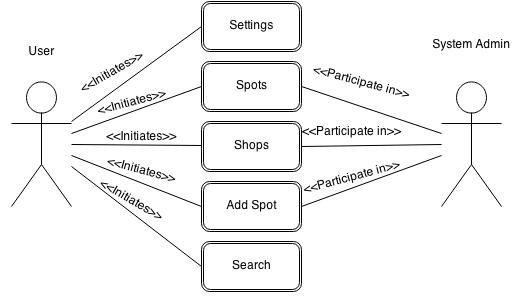
\includegraphics[scale = 0.75]{usecasemodel}
\end{center}
\end{figure}

Højniveau diagram der skal illustrere de forskellige aktører\\\\
Som det ses er der 2 aktører, brugeren og Ejeren. Brugeren kan benytter de forskellige funktioner i appen, og ejeren redigere og kontrollere uploads og spots. 
\pagebreak\\
\textit{(c) Tre specificerede use cases, som er særlig vigtige i jeres system}\\
\setlength\parindent{0pt}
\section*{Use-cases}
\subsection*{Få information om et spot}
\hrule\vspace{5mm}
\textit{Use case name:} FindSpot\\
\hrule\vspace{5mm}
\textit{Actor:} en bruger der gerne vil finde information om et spot\\
\hrule\vspace{5mm}
\textit{Entry condition:} brugeren åbner appen\\
\hrule\vspace{5mm}
\textit{Flow of events:}
\begin{enumerate}
\item Brugeren bliver præsenteret for et kort med sin egen positition i centrum og en menu linje i toppen
\item Brugeren trykker på en "marker" på kortet for det spot han vil se information.
\end{enumerate}
\hrule\vspace{5mm}
\textit{Exit condition:} Brugeren ser nu et pop-up vindue med information om spottet.\\
\hrule\vspace{5mm}
\newpage
\subsection*{Tilføj spot}
\hrule\vspace{5mm}
\textit{Use case name:} AddSpot\\
\hrule\vspace{5mm}
\textit{Actor:} en bruger der gerne vil tilføje et spot\\
\hrule\vspace{5mm}
\textit{Entry condition:} brugeren åbner appen\\
\hrule\vspace{5mm}
\textit{Flow of events:}
\begin{enumerate}
\item Brugeren trykker på knappen "Add spot", der sender ham videre til en udfyldelses formular
\item Brugeren udfylder formularen og gemmer denne, formularen sendes derefter til godkendelse hos administratoren
\end{enumerate}
\hrule\vspace{5mm}
\textit{Exit condition:} Brugeren sendes retur til forsiden\\
\hrule\vspace{5mm}
\newpage
\subsection*{Ændre indstillinger}
\hrule\vspace{5mm}
\textit{Use case name:} ChangeCondition\\
\hrule\vspace{5mm}
\textit{Actor:} en bruger der gerne vil ændre indstillingerne\\
\hrule\vspace{5mm}
\textit{Entry condition:} brugeren åbner appen\\
\hrule\vspace{5mm}
\textit{Flow of events:}
\begin{enumerate}
\item Brugeren trykker på indstillinger, der sender brugeren videre til en ny side
\item Brugeren bliver præsenteret for de forskellige indstillinger han kan vælge
\item Når brugeren han ændret indstillinger er der en ok knap som tilføjer indstillingerne
\end{enumerate}
\hrule\vspace{5mm}
\textit{Exit condition:} Indstillingerne er nu i funktion og brugeren sendes tilbage til forsiden\\
\hrule\vspace{5mm}
\pagebreak

\textit{(d) Et klassediagram over jeres problemområde (solution-domain)}\\\\
\begin{figure}[h]
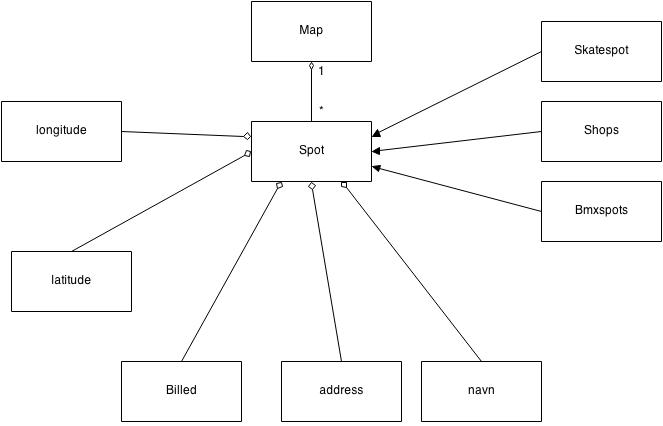
\includegraphics[scale = 0.5]{classdiagram}
\end{figure}\\\\
\newpage
\textit{(e) Sekvens-diagrammer over de 3 use-cases specificeret i punkt (c)}\\
Husk at alle diagrammer skal være fulgt af tekstbeskrivelser, der gør diagrammerne fuldt
forståelige også for læsere uden særligt domænekendskab.\\
\begin{figure}[h]
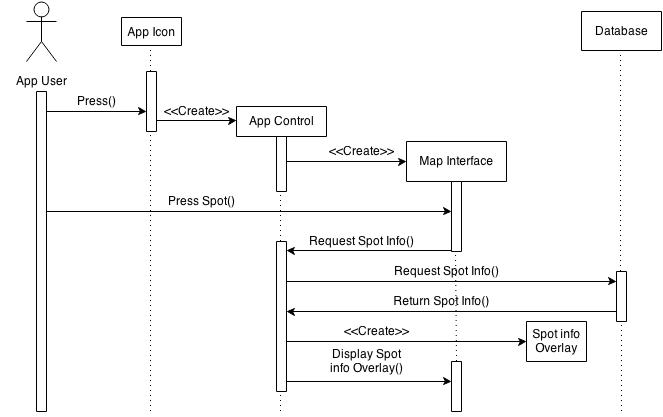
\includegraphics[scale = 0.5]{sekdia1}
\end{figure}

Sekvensdiagram over find spot information:\\
Brugeren starter App'en på sin telefon. App'en viser kort interfacen og brugeren vælger et spot fra kortet. 
App'en henter spot informationerne fra database og viser dem i et overlay.
\newpage

\begin{figure}[h]
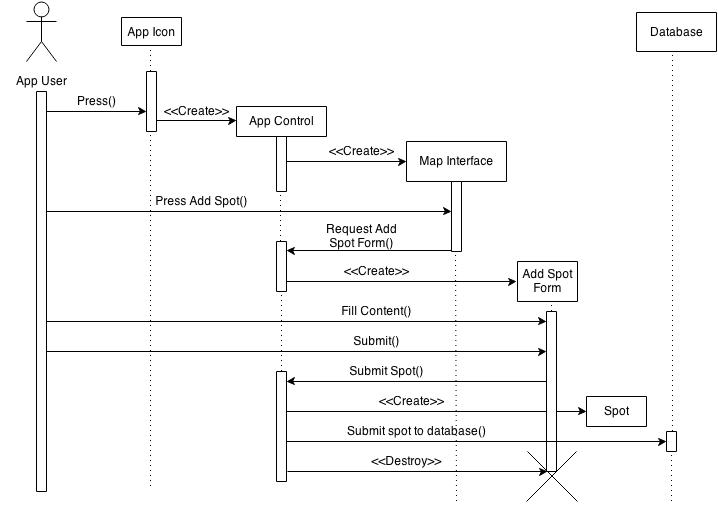
\includegraphics[scale = 0.5]{sekdia2}
\end{figure}

Sekvensdiagram over add spot funktionen:\\
Brugeren starter App'en på sin telefon. App'en viser kort interfacen og brugeren vælger add spot fra menuen.
App'en viser en add spot formular. Brugeren udfylder formularen med spot informationerne og submiter den.
App'en sender spotet til databasen.

\newpage

\begin{figure}[h]
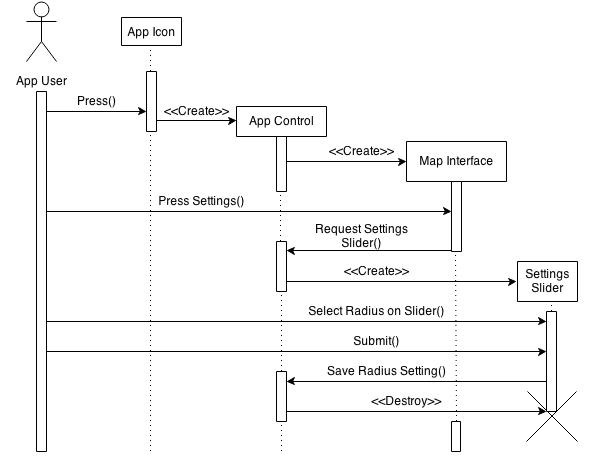
\includegraphics[scale = 0.5]{sekdia3}
\end{figure}

Sekvensdiagram over indstillinger:\\
Brugeren starter App'en på sin telefon. App'en viser kort interfacen og brugeren vælger settings fra menuen.
App'en viser en radius slider. Brugeren vælger en radius og og submiter den. App'en gemmer den nye radius.


\pagebreak

\section{Systemdesign sammenfatning}
\textit{Kapitlet resumerer jeres foreløbige system-design så kort og klart som muligt. Samtidig
udpeger I de vigtigste udestående design- og implementationsopgaver}.\\

Vores plan vedrørende udviklingen af appen har indtil nu, været at bygge appen op i java med android developer tools. Det gav os en del udfordring, da vi ikke kunne få den simpleste udgave til at køre på en simulator. De mange timer og forsøg har gjort at vi følte os nødsaget til at gøre projektet mindre omfattende. 
\\\\
Derfor har vi valgt at bygge applikationen op webbaseret i html, css, javascript og mySQL, hvilket er programmer og metoder vi har erfaring med i forvejen. 
Hele implementeringen af Google maps foregår med javascript(altså som en hjemmeside), hvor vi så bagefter vil lave en android webview app, så vi kan tilføje applikationen på google play store. vi mangler at implementere alt andet end kortet på nuværende tidspunkt.

\section{Program- og systemtest}
\textit{Dokumenter jeres foreløbige test af IT-løsningen. I kapitlet sammenfattes hovedresultaterne af
jeres test-aktiviteter; mens test plan, test case specification, test incident report og test report
summary placeres som bilag}.\\\\
Vi har tænkt os at teste det ved at få nogen mennesker til at lave think-aloud mens de prøver hjemmesiden. Dette kommer snart til at ske og vil være med i delrapport 3. Derudover vil vi selfølgelig selv teste løbenede på diverse funktioner som vi får lavet til hjemmesiden for at sikre os at det kører som det skal.
\pagebreak
\section{Brugergrænseflade og interaktionsdesign}
\textit{(a) Præsenter skærmbilleder af de mest interessante dele af jeres brugergrænseflade}

\begin{figure}[h]
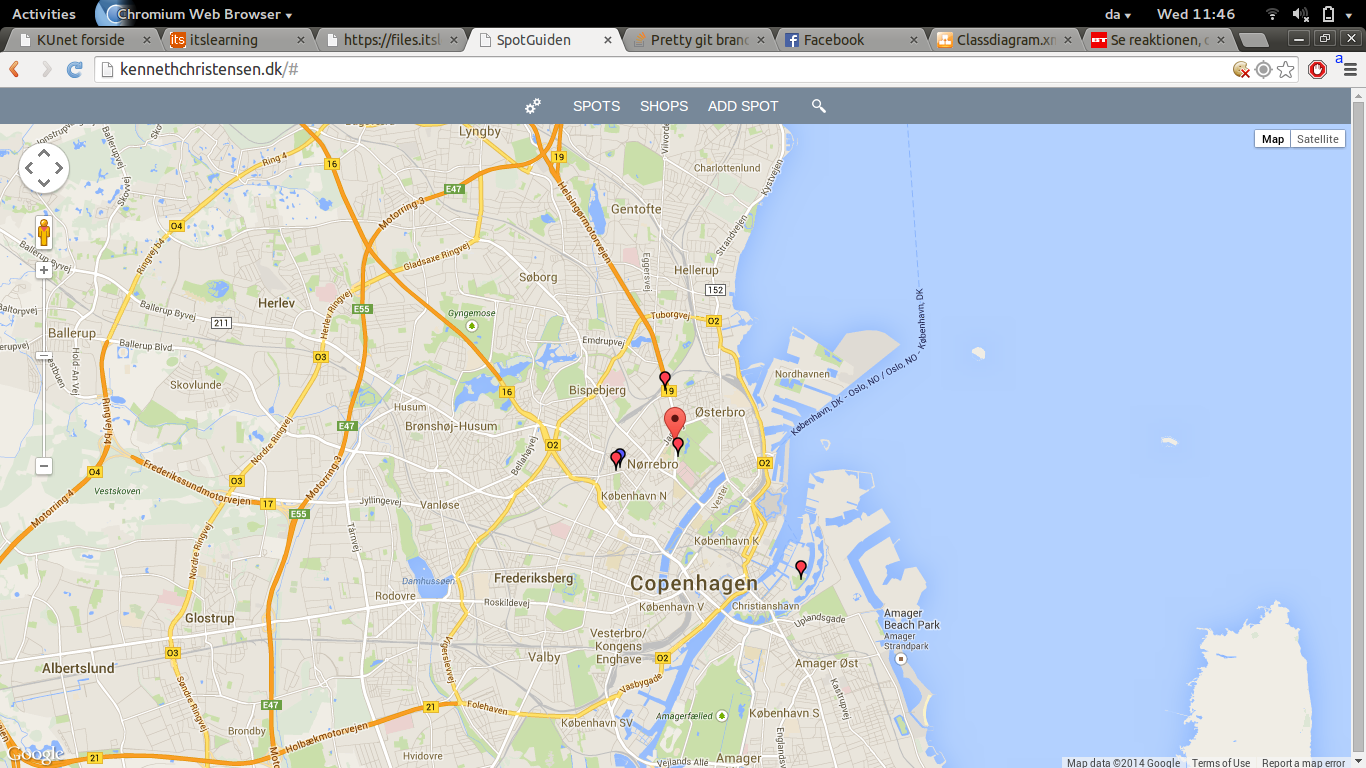
\includegraphics[scale = 0.3]{screen1}
\end{figure}

Billedet viser vores foreløbige hjemmeside der blot indeholder en menu uden funktioner, samt et kort med "spots" på den måde som vi vil præsentere dem. \\ \\
Settings: 
\begin{figure}[h]
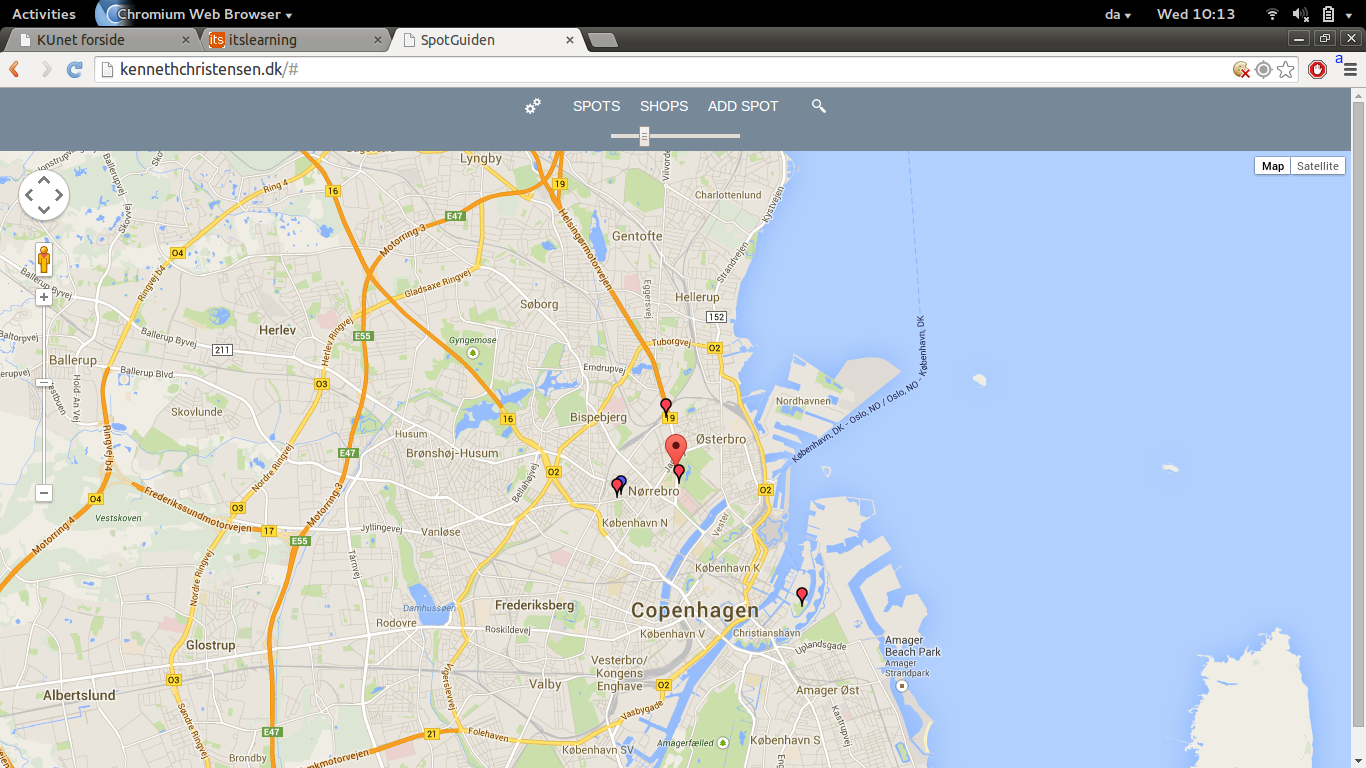
\includegraphics[scale = 0.21]{slider}
\end{figure}\\
Når man trykker på settings kommer der en slider, som der kan bestemme hvor stor en radius siden skla loade spots fra, vurderet fra brugerens nuværende position.\\\\
Spots: 
Når du trykker her kommer der en liste frem over alle de forskellige spots som man herefter trykke på dem. Dette vil centrerer dem på kortet.\\\\
Shops: \\
Centrerer kortet på BMXButikken.\\ \\
Add spot:
\begin{figure}[h]
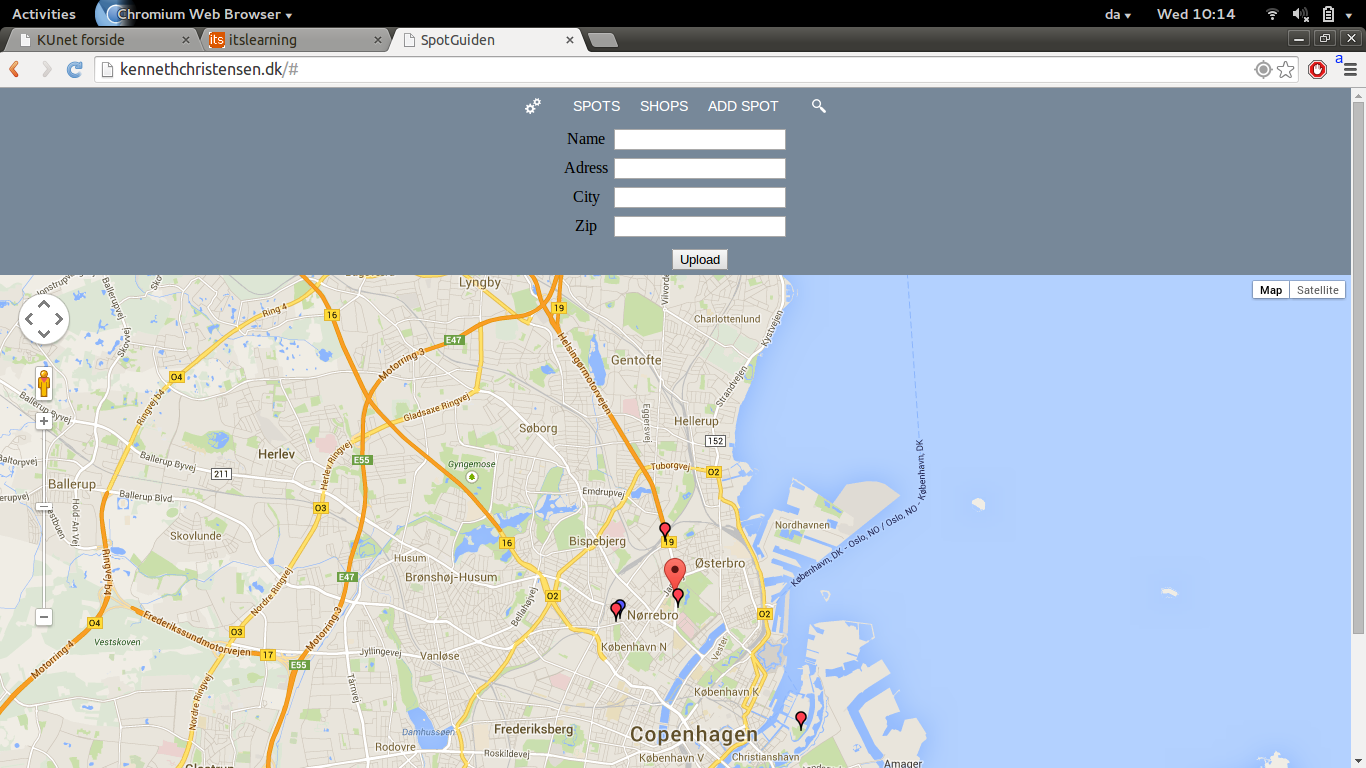
\includegraphics[scale = 0.21]{Addspot}
\end{figure}\\ 
Når der trykkes på dette kommer der en formular frem som man skal udfylde med: Name, Address, City, zip og billede.\\
\pagebreak
Search: 
\begin{figure}[h]
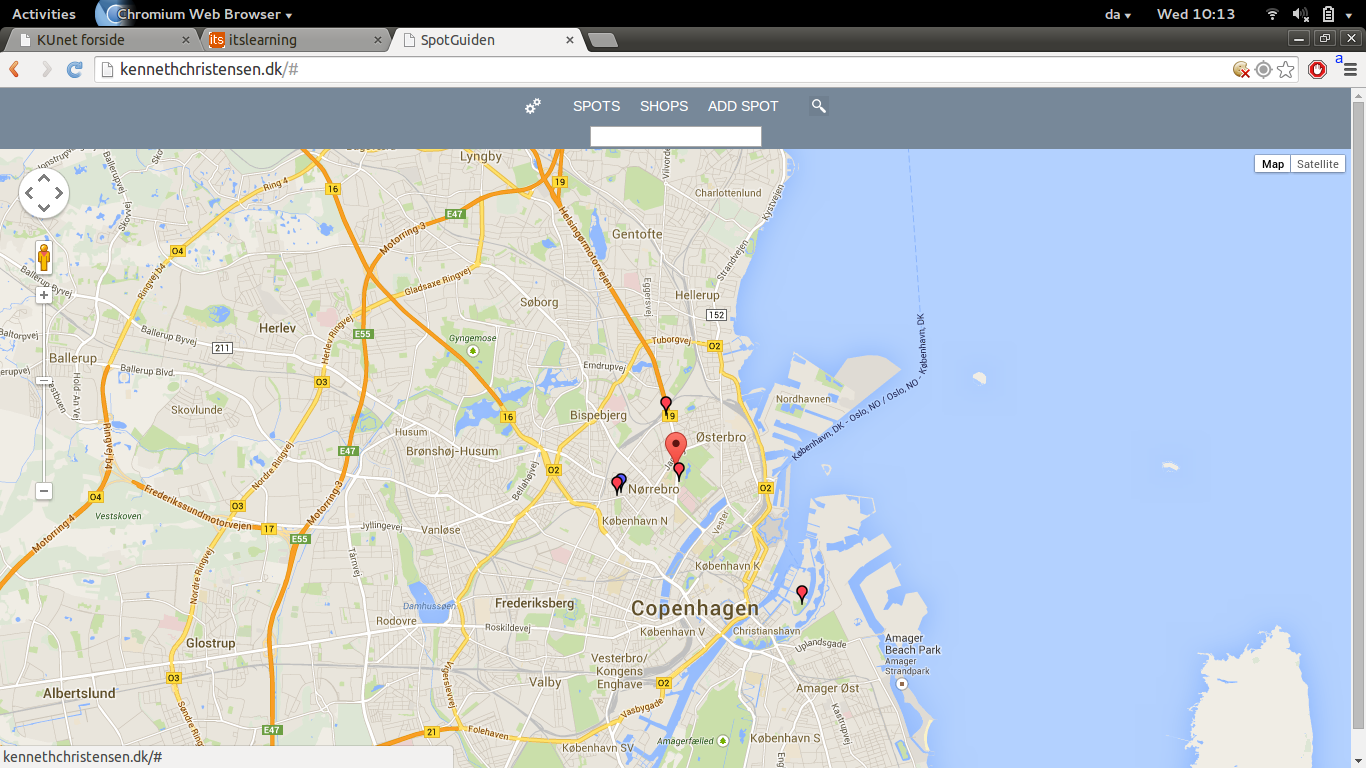
\includegraphics[scale = 0.21]{Search}
\end{figure}\\
Kommer frem med et søgefelt hvor man kan søge på spots via navn/zipcode/by.\\

\textit{(b) Illustrer flowet/dynamikken i brugerinteraktionen mellem skærmbillederne}\\\\
Dette vil blive udfyldt i delrapport 3 eller 4 hvor vi er kommet længere med programmet.\\\\
\textit{(c) En audio-visuel præsentation af brugergrænsefladen af den seneste kørende prototype}\\\\
Dette punkt vil vi udfylde til delrapport 4 da vores projekt gerne skulle være færdig eller have mere funktionalitet på dette tidspunkt
\newpage
\textit{(d) Resultatet af seneste tænke-højt forsøg gennemført med een eller flere af jeres brugere}
\subsection{Tænk højt øvelser}
Jesper: Find det spot nærmest dig.\\
Umiddelbart kan jeg se at jeg er den store pil, og lige ved siden af den store pil er der en lille pil, så den vil jeg prøve at trykke på, hov der åbnede et vindue hvor der står fælledparken.\\\\
Sebastian: Find Bmxbutikkens marker på kortet\\
Jeg prøver at trykke på en rød først og kan se at det er en skatepark, så jeg prøver den blå pil og der var bmxbutikken.\\\\
Kenneth: Ændrer indstillingerne.\\
Der er 2 tandhjul det må være indstillinger, så der trykker jeg og så kan jeg trække frem og tilbage på slideren og se flere eller færre spots.\\\\

\pagebreak
\section{Versionstyring}
\textit{Som bilag skal vedlægges jeres nuværende commit-log samt jeres
programkode. Kommentér kort (ca 1/2 side) de vigtigste ændringer, der er sket i programkoden}\\

Vi har nu fået opdateret vores hjemmeside så istedet for der står settings og search er der nu kommet to forskellige ikoner som alle brugere kender, forstørrelsesglas og tandhjul. Der er ikke kommet noget funktionalitet bag det men designet til disse to knapper er nu kommet på. \\
Vi har fået opdateret vores database med flere spots og gjort det muligt for vores hjemmeside at der sker noget når der bliver trykket på en marker. Det der sker nu er at der kommer et info vindue op, med en addresse og et billede af spottet.\\
Vores app til at kunne køre hjemmesiden på android er næsten færdig.\\
Det eneste problem vi har omkring dette er at den ikke er kompatibel med at få en brugers position men dette vil altid blive et problem når nu den skal køre kunne køre offline.\\
Vores midlertidige projekt kan ses på \url{www.kennethchristensen.dk} det kan godt det stemmer over med hvad vi har beskrevet i rapporten da der stadig arbejdes videre på det.\\

\pagebreak
\section{Projektsamarbejdet}
\textit{Beskriv konkret og oplysende hvordan det går med samarbejdet med brugerne
og med arbejdet internt i gruppen. Herunder skal bl.a. oplyses antallet af møder med brugerne under
projektforløbet (fx på en tidslinje), mødeformen i gruppen, samt hvorledes jeres referat- og
dokumentationsform fungerer. Hvorledes prioriterer og styrer I projektindsatsen, så I sikrer
fremdrift på de felter, som er mest risikable/afgørende for et succesfuldt resultat? Herunder, beskriv
og diskuter:}\\

\textit{(a) Hvad går godt?}\\
Det interne arbejde i gruppen fungerer godt. Alle medlemmer i gruppen deltager aktivt, engageret og møder til tiden på de aftalte møde dage. Selve arbejdet prøver vi at fordele imellem os alt efter interesse og det sikrer en god stabil arbejds indsats.\\

\textit{(b) Hvad går mindre godt?}\\

Vi har haft uventede problemer hvad angår systemdesignet da vi har måttet ændre kurs og gå over i en webbaseret udgave. Det har betydet at vi har haft nogle arbejdsspildtimer og vi er derfor ikke noget helt så langt som planlagt.\\

\textit{(c) Hvad vil I gøre for at effektivisere jeres udviklingsarbejde?}\\

I det vi tog skridtet fra android app til webbaseret app, har vi taget de første skridt i effektiviseringen. Derudover regner vi med at kunne begynde at arbejde selvstændigt på enkelte dele af systemet når vi har fået den første prototype helt op at køre. Det skullle bevirke at det bliver nemmere for de enkelte individer i gruppen at få plads i deres skema, til at få arbejdet på projektet og dermed få arbejdet flere timer. 

\pagebreak
\section{Review}
\subsection{Cardboard computers: Mockingit- up or hands-on the future.}

Artiklen handler om forholdet mellem computere og 'mennesket' som bruger dem. Artiklen argumentere for at computere skal forstås gennem mennesket brug af dem. Forfatteren starter med et hurtigt eksempel om en journalistisk process og hvordan et mock-up af et arbejdsmiljø, hvor computere er involveret, kan hjælpe med at påvirke arbejds-processen positivt.\\
'Why mock it up?' og 'We did not make it up'\\
Artiklen forklarer hurtigt hvorfor at lave mock-ups er en gode ide. Det gør det nemt for den endelig bruger at forstå hvordan det endelig produkt kommer til at fungere, og gør det nemmere at involvere brugeren i design processen. Derudover er det billigt så man kan lave en masse forsøg for at finde det som fungere bedst. Det bliver også pointeret at mock-ups ikke er noget nyt, da vi typisk som børn bruger mock-ups i form af legetøjs-biler, dukker osv. Det er også brugt i industriel design til at skabe gode og arbejdsvenlige arbejdspladser. \\
'Language games' og 'hands-on Experiences and Ready-to-hand Use'\\
Artiklen gør, i dette kapitel, det klart at det er vigtigt at alle involveret i et mock-up taler samme 'sprog', forstået på den måde at alle er klar over hvad hver ting repræsenterer og hvordan interaktion med objekter fungere. Forfatterne kommer så med et eksempel fra deres egen erfaring, hvor de havde udarbejdet en meget omfattende og detaljeret beskrivelse af det pågældende system. Dette kunne brugerne ikke relatere til. Det blev løst ved bruge et mock-up, hvor brugerne kunne bruge systemet i deres naturlige miljø og derved relatere til det.\\
'Beyond the Cardboard Computer', 'Second Generation Mock-ups' og 'Simple Mock-ups: Advantages and Disadvantages'\\
Artiklen gennemgår i disse kapitler hvad man kan gøre for at gøre sine mock-ups mere detaljeret, så som at bruge video eller slideshows. Man skal være opmærksom på at de ting bruger skal være almen-kendte så de holder sig inde for 'sproget'. En grund til at bruge simple mock-ups kan være pris begrænsninger, da store investeringer tidligt i design-processen typisk ikke er en god ide.\\
'Computers in Mock-ups: Overcoming the Disadvantages' og 'Computers in Mock-ups: Losing the Advantages?'\\
Artiklen dækker herefter fordelene ved at bruge computere til sit mock-up. F.eks at det er nemt at gemme et layout af sit mock-up og derefter afprøve andre layout uden at miste noget af det oprindelige. Dette kræver dog at dem som involveret i mock-upet har kendskab til computere. Ved brug af computere i mock-upet bliver det også muligt at dække spørgsmål rettet mere mod programmet (interface) mod ved brug af papkasser o.lign. En ulempe ved den forhøjet funktionalitet computere giver, er at brugerne muligvis tror at mock-upet er et stort set færdigt produkt, men da dette ikke er tilfældet kan der opstå forvirring og misforståelser.\\

Det vi i gruppen mener der er værd at tage med fra denne artikel er selve ideen om at simplificere ens system ned til et punkt, hvor det er muligt for den fremtidige bruger at kunne deltage. Det nytter ikke at snakke om f.eks kode hvor brugeren ikke kan bidrage med noget. Med et program vil dog være knapt så nyttigt at lave en hel arbejds-station (i pap), men derimod bruge f.eks et story-board til at gøre tingene forståelige for ikke programmøre. Story-boardet vil dog være bedst at lave på computer for at gøre rettelse o.lign nemmere og mindske risikoen for at miste materiale.

\pagebreak
\subsection{No Silver Bullet}

"No Silver Bullet - Essence and Accidents of Software Engineering" er en artikel omkring software udvikling, skrevet af Fred Brooks i 1986. Brooks starter ud med at tilsidesætte software udvikling med myten om en varulv. Den eneste måde at få bugt med en varulv er som bekendt ved at bruge en "silver bullet". Brooks mener imidlertid  at  "there is no single development, in either technology or management technique, which by itself promises even one order of magnitude improvement within a decade in productivity, in reliability, in simplicity.". Han fortsætter i samme dur med "we cannot expect ever to see two-fold gains every two years" in software udvikling, ligesom tilfældet har været indenfor hardware udvikling. Dermed konstaterer han at denne såkaldte "silver bullet" ikke eksisterer og ikke vil blive udviklet indenfor de næste 10 år.\\\\
I følge Brooks kan grunden til at denne "silver bullet"  ikke findes, deles op i to problemer henholdsvis "Essence complexity - Bliver skabt af det problem der skal løses og kan altså ikke fjernes" og "Accidents complexity - Der opstår på grund af fejl udvikleren laver og som dermed kan rettes". Men samtidig hævder han at software udviklerer på dette tidspunkt(1986) bruger det meste af sin tid på "Essence complexity", og mener altså at selvom "Accidential activities" elimineres vil det ikke resulterer i en "magnitude improvement" (Tifoldig forbedring i udviklings hastigheden).  \\\\
Selvom der bliver heftigt argumenteret for at der ikke findes en "silver bullet" mener Brooks alligevel er der er et par lyspunkter på vej, bla. i form af høj niveau programmerings sprog som Fortran, der kan sammenlignes lidt med nutidens C og Java. \\\\
Brooks proklamerer yderligere at der er forskel på gode system udviklere og fantastiske, idet at han mener software udviling er en kreativ process og at nogle udviklerer er grundlæggende bedre end andre, grundet deres genetiske arv. At udnytte dette og sørge for at skabe fantastiske udviklere fremfor midelmådige skulle ifølge Brooks kunne lede til en "magnitude improvement".\\\\
\newpage

\noindent\textbf{Artiklen set i forhold til object orienteret programmering}\\\\
Brooks nævner blandt andet at han er stor fortaler for object orienteret programmering og ser store muligheder i udviklingen af dette. Han mener at OOP, sammen med et høj niveau programmerings sprog, kunne resulterer i at mindske både "accidential complexity" og "essentual complexity" og dermed være en mulig "silver bullet".\\\\
Vi (gruppen), mener imidlertid ikke at dette er tilfældet da kompleksiteten ikke kan simpliciferes ved hjælp af disse værktøjer, men blot bedre kontrolleres. Vi ser derfor OOP som en teknologi, et koncept altså en måde at angribe et givent problem på. Konceptet tilbyder værktøjer der kan forbedrer et design og derigennem gøre det nemmere at håndterer kompleksiteten, men udvikleren kan ligeså godt ende med et dårligt design der forværrer problemet og dermed kompleksiteten. Så kort sagt, hvis ikke konceptet bruges "rigtigt", risikerer du blot at yderligere besværliggøre opgaven. Vi konstaterer derfor at OOP ikke er en løsning til kompleksitet, men et (af flere) redskaber til at kontrollerer det, hvis udvikleren evner dette.
\pagebreak
\section{Bilag}

\subsection{Commitlog}
* <73f7798> 2014-05-14 [mhejselbak]  (HEAD, master) delrapport 3 tilføjet \\
* <8fff4f0> 2014-05-14 [mhejselbak]  delrapport 3 tilføjet \\
* <a9c842d> 2014-05-08 [rasmus03]  (origin/master, origin/HEAD) Genupload af delrapport \\
* <d58b7ea> 2014-05-08 [mhejselbak]  Delrapport 2 genafl tilfoejet \\
* <2572462> 2014-05-08 [rasmus03]  Tilføjede en ny usecasemodel \\
* <04acdab> 2014-05-07 [rasmus03]  Mindre opdateringer til delrapport 2 - intet nyt \\
* <533b5cb> 2014-05-07 [mhejselbak]  added more to part 5 \\
* <c5d6de6> 2014-05-07 [runefranch]  updateret delrapport \\
* <c4bdcc5> 2014-05-07 [rasmus03]  Opdaterede delrapport 2 med nye sekvensdiagrammer \\
* <e4f926b> 2014-05-07 [rasmus03]  Tilføjede gruppe reviews (igen) \\
*   <a8c5bbd> 2014-05-07 [runefranch]  Merge branch 'master' of https://github.com/mhejselbak/PKSU \\
|\textbackslash   \\
* | <95229b4> 2014-05-07 [runefranch]  Sekvens diagram \\
| * <d3ad6bd> 2014-05-07 [rasmus03]  Flyttede log.log til den rette mappe\\
|/  \\
* <a0eb8ab> 2014-05-07 [mhejselbak]  Deleted style.css and edited delrapport2 \\
* <3db9ac0> 2014-05-07 [rasmus03]  Opdaterede tekst i delrapport 2 \\
* <b4614f0> 2014-04-28 [mhejselbak]  CSS til hjemmeside \\
* <d0c4133> 2014-04-28 [rasmus03]  Tilføjede første udlæg til den webbaserede android application \\
* <ba05d40> 2014-04-28 [rasmus03]  Tilføjede vores review af “Mood” \\
* <1da40ab> 2014-04-24 [rasmus03]  Updaterede filer til delrapport 2 \\
* <89ae7a4> 2014-04-24 [rasmus03]  Commitlog billede \\
* <6f57d2e> 2014-04-24 [rasmus03]  Tilføjede vores udkast til hjemmesiden \\
* <2077057> 2014-04-24 [runefranch]  Nyt sekvens diagram \\
* <a006ca4> 2014-04-24 [runefranch]  sidste sekvens diagram \\ 
* <f2ad5a2> 2014-04-23 [rasmus03]  Updated files and added screenshots \\
* <c201cd9> 2014-04-23 [runefranch]  sekvens diagram \\
* <ee33ad2> 2014-04-23 [rasmus03]  Opdaterede delrapport2 med 2/2 review og use-cases. \\
* <592de43> 2014-04-23 [runefranch]  reviewartikel \\
* <e77b576> 2014-04-23 [rasmus03]  FACTOR model - Bruges i delrapport 2 \\
* <599276d> 2014-04-23 [rasmus03]  Delrapport 2 - Består af punkt 1, 2 og 1/2 review \\
* <b2271ec> 2014-04-22 [mhejselbak]  Prototype \\
* <6e1b71b> 2014-04-10 [runefranch]  review update \\
* <d81beae> 2014-04-09 [runefranch]  Review \\
* <19705bc> 2014-04-03 [mhejselbak]  Initial commit \\
\subsection{Referater}

\subsection*{Referat fra sidste møde med kunde}
Møde med Travis den 8/6 \\
Vi mødtes med travis i bmxbutikken eller som deres butik på nørrebrogade hedder "pedal \& Co" Her fremviste vi vores program til ham og snakkede om forbedringer og evt ekstra funktionalitet, vi diskuterede også hvilken slags spots der skulle op og om man evt. skulle holde nogle spots hemmelige for brugerene for at ikke opfordre små børn til at hoppe over hegn f.eks.\\
Han var rigtig tilfreds med resultatet af programmet indtil videre, og glædede sig til at det blev færdig, så han kunne få det ud til den danske bmx scene. Han havde dog også nogle ting, som han synes vi skulle tænke ekstra over. Han synes bla. ikke at hjemmesiden var helt inuitiv nok han kom med et eksempel med den lille gule mand og google street view, hvor at en erfaren bruger af google maps ved at man skal trække den gule mand ned på kortet, vil en bruger der ikke er vand til google maps ikke kende den funktionalitet. Derfor ville han gerne have en knap inde i infowindows med streetview, så en bruger af appen også trykke på en knap indei  infowindowet og se googles billeder af spottet.\\
Derudover snakkede vi også om at få brugere til at bruge hjemmesiden, hvor vi blev enige om at det var vigtigt at starte med en database med en del spots, simpelthen for at få brugerne til at bruge hjemmesiden. Derudover hvis der først er brugere på siden vil de forhåbentlig også selv uploade deres egne lokale spots og på den måde kan spotguiden udvide sig til at være national, da der kommer massere af bmx'ere og skatere fra Jylland til hovedstaden for at køre
\end{document}